%%%%%%%%%%%%%%%%%%%%%%%%%%%%%%%%%%%%%%%%%
% Proceedings of the National Academy of Sciences (PNAS)
% LaTeX Template
% Version 1.0 (19/5/13)
%
% This template has been downloaded from:
% http://www.LaTeXTemplates.com
%
% Original author:
% The PNAStwo class was created and is owned by PNAS:
% http://www.pnas.org/site/authors/LaTex.xhtml
% This template has been modified from the blank PNAS template to include
% examples of how to insert content and drastically change commenting. The
% structural integrity is maintained as in the original blank template.
%
% Original header:
%% PNAStmpl.tex
%% Template file to use for PNAS articles prepared in LaTeX
%% Version: Apr 14, 2008
%
%%%%%%%%%%%%%%%%%%%%%%%%%%%%%%%%%%%%%%%%%

%----------------------------------------------------------------------------------------
%	PACKAGES AND OTHER DOCUMENT CONFIGURATIONS
%----------------------------------------------------------------------------------------

%------------------------------------------------
% BASIC CLASS FILE
%------------------------------------------------

%% PNAStwo for two column articles is called by default.
%% Uncomment PNASone for single column articles. One column class
%% and style files are available upon request from pnas@nas.edu.

%\documentclass{pnasone}
\documentclass{pnastwo}

%------------------------------------------------
% POSITION OF TEXT
%------------------------------------------------

%% Changing position of text on physical page:
%% Since not all printers position
%% the printed page in the same place on the physical page,
%% you can change the position yourself here, if you need to:

% \advance\voffset -.5in % Minus dimension will raise the printed page on the 
                         %  physical page; positive dimension will lower it.

%% You may set the dimension to the size that you need.

%------------------------------------------------
% GRAPHICS STYLE FILE
%------------------------------------------------

%% Requires graphics style file (graphicx.sty), used for inserting
%% .eps/image files into LaTeX articles.
%% Note that inclusion of .eps files is for your reference only;
%% when submitting to PNAS please submit figures separately.

%% Type into the square brackets the name of the driver program 
%% that you are using. If you don't know, try dvips, which is the
%% most common PC driver, or textures for the Mac. These are the options:

% [dvips], [xdvi], [dvipdf], [dvipdfm], [dvipdfmx], [pdftex], [dvipsone],
% [dviwindo], [emtex], [dviwin], [pctexps], [pctexwin], [pctexhp], [pctex32],
% [truetex], [tcidvi], [vtex], [oztex], [textures], [xetex]

\usepackage{graphicx}

%------------------------------------------------
% OPTIONAL POSTSCRIPT FONT FILES
%------------------------------------------------

%% PostScript font files: You may need to edit the PNASoneF.sty
%% or PNAStwoF.sty file to make the font names match those on your system. 
%% Alternatively, you can leave the font style file commands commented out
%% and typeset your article using the default Computer Modern 
%% fonts (recommended). If accepted, your article will be typeset
%% at PNAS using PostScript fonts.

% Choose PNASoneF for one column; PNAStwoF for two column:
%\usepackage{PNASoneF}
%\usepackage{PNAStwoF}

%------------------------------------------------
% ADDITIONAL OPTIONAL STYLE FILES
%------------------------------------------------

%% The AMS math files are commonly used to gain access to useful features
%% like extended math fonts and math commands.

\usepackage{amssymb,amsfonts,amsmath}

%------------------------------------------------
% OPTIONAL MACRO FILES
%------------------------------------------------

%% Insert self-defined macros here.
%% \newcommand definitions are recommended; \def definitions are supported

%\newcommand{\mfrac}[2]{\frac{\displaystyle #1}{\displaystyle #2}}
%\def\s{\sigma}

%------------------------------------------------
% DO NOT EDIT THIS SECTION
%------------------------------------------------

%% For PNAS Only:
\contributor{Future Submission to Proceedings of the National Academy of Sciences of the United States of America}
\url{www.pnas.org/cgi/doi/xxx}
\copyrightyear{x}
\issuedate{Issue Date}
\volume{Volume}
\issuenumber{Issue Number}

%----------------------------------------------------------------------------------------

\begin{document}

%----------------------------------------------------------------------------------------
%	TITLE AND AUTHORS
%----------------------------------------------------------------------------------------

\title{Co-evolution of strategic decision making: DOTA 2 as a proxy for cybersecurity environments} % For titles, only capitalize the first letter

%------------------------------------------------

%% Enter authors via the \author command.  
%% Use \affil to define affiliations.
%% (Leave no spaces between author name and \affil command)

%% Note that the \thanks{} command has been disabled in favor of
%% a generic, reserved space for PNAS publication footnotes.

%% \author{<author name>
%% \affil{<number>}{<Institution>}} One number for each institution.
%% The same number should be used for authors that
%% are affiliated with the same institution, after the first time
%% only the number is needed, ie, \affil{number}{text}, \affil{number}{}
%% Then, before last author ...
%% \and
%% \author{<author name>
%% \affil{<number>}{}}

%% For example, assuming Garcia and Sonnery are both affiliated with
%% Universidad de Murcia:
%% \author{Roberta Graff\affil{1}{University of Cambridge, Cambridge,
%% United Kingdom},
%% Javier de Ruiz Garcia\affil{2}{Universidad de Murcia, Bioquimica y Biologia
%% Molecular, Murcia, Spain}, \and Franklin Sonnery\affil{2}{}}

\author{A. L. Sallaska\affil{1}{The MITRE Corporation},
D. Biro\affil{2}{Albert Einstein College of Medicine},
S. Duran\affil{3}{Pompeu Fabra University},
\and
M. Stuart\affil{4}{University of California, Berkeley}}

\contributor{Submitted to Proceedings of the National Academy of Sciences
of the United States of America}

%----------------------------------------------------------------------------------------

\maketitle % The \maketitle command is necessary to build the title page

\begin{article}

%----------------------------------------------------------------------------------------
%	ABSTRACT, KEYWORDS AND ABBREVIATIONS
%----------------------------------------------------------------------------------------

\begin{abstract}
Computer hackers use certain strategies to penetrate systems.  These strategies evolve over time, usually in response to the defense mechanisms employed by the system administrators.  Being able to identify the strategies and when they change is of paramount importance to ensure the safety of the systems.  Because data to help this effort is scarce, this paper explores the possibility of using competitive, strategic video game data as a proxy to identify strategies and their change points.  




\end{abstract}

%------------------------------------------------

\keywords{Cybersecurity | Intrusion detection algorithms | adaptive strategies | video game data} % When adding keywords, separate each term with a straight line: |

%------------------------------------------------

%% Optional for entering abbreviations, separate the abbreviation from
%% its definition with a comma, separate each pair with a semicolon:
%% for example:
%% \abbreviations{SAM, self-assembled monolayer; OTS,
%% octadecyltrichlorosilane}

% \abbreviations{}
\abbreviations{DOTA, Defense of the Ancients}

%----------------------------------------------------------------------------------------
%	PUBLICATION CONTENT
%----------------------------------------------------------------------------------------

%% The first letter of the article should be drop cap: \dropcap{} e.g.,
%\dropcap{I}n this article we study the evolution of ''almost-sharp'' fronts

\section{Introduction}

Existing performance metrics of cyber intrusion detection algorithms, such as false positive or negative rates, are unable to capture the level of granularity necessary to significantly improve the algorithms, especially when a single, definitive outcome is rarely the case for this domain.  Traditional static cyber defense systems also require long lead times to install patch updates, and staving off damage in real time is unfeasible using these metrics.  Therefore, metrics must evolve to provide real-time evaluations of adaptive adversaries whose strategies may change depending on the protective mechanisms they encounter, as well as characterizing sequences of detections.  

Usable data from within the cyber domain that may help to strengthen detection algorithm scoring is nearly nonexistent.  If actual attacks are documented in the real world, this data is rarely made available and may be network specific (hence, not generalizable).   Thus, a proxy for the data is necessary.  An online battle arena video game called Defense of the Ancients 2 (DOTA 2) is a rich data source of real-time adaptive adversaries.  DOTA 2 is a strategic, competitive, multiplayer game where two teams of five individuals each compete against each other to complete objectives and to destroy the other team?s base in a time frame of $\sim$ 20 to $\sim$ 90 minutes.  The players deploy various in-game and between-game tactics and procedures to achieve a specific measurable objective.  Professional players vie for tens of millions of dollars in prize pools each year, and over 2 billion games have been played.  The results in this paper are using data from a cache of 500 GB of aggregated game data ($\sim$ 2.5 million games played over one year) and from X GB of raw, event-by-event data.  Our goal is to use this data to shed light on how we can 1) detect and 2) quantify the rate of change of strategies in co-evolutionary systems.  

This is akin to the classic `Red Queen hypothesis' in evolutionary biology, but in this case we are interested in human behaviors where a strategy can be considered most generally as a `meme' of sorts.  Our hypotheses include: 1) a mapping exists between game observables and a set of strategies, 2) a measurable signal can be extracted from which to ascertain the adoption, stabilization, and decay of specific strategy traits, 3) changes in strategies occur over time, and 4) strategy changes are driven (at least in part) from behaviors of the opposing team.  We postulate that testing these hypotheses will require an understanding of the co-evolutionary dynamics of the overall environment.  In particular, the human behavioral components underlying the adversary/defense team actions will need to be assessed.  The use of data from a multiplayer online game for this purpose assumes there is a valid mapping between the `game-space' to `cyber-space' behaviors from which useful inferences can be made.  Through this exercise we hope to understand what types of data (if any) are useful for this purpose and how one might develop proxies to characterize strategies.  Ultimately, we hope that the analysis could be applied against realistic data specific to a cyber intrusion.  

\section{The Game: DOTA 2}

An aerial view of the DOTA game board is shown in Fig.~\ref{gameboard}.  The goal of the game is to destroy the opposing team's base, their Ancient, located either in the lower left or upper right corner of the figure.  

\begin{figure}[h]
\centerline{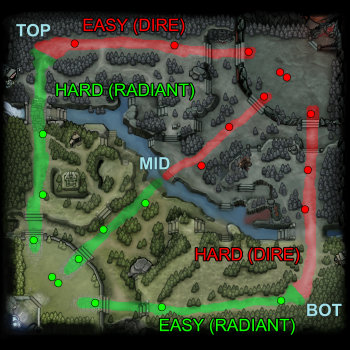
\includegraphics[width=.8\linewidth]{./Figs/GameBoard.png}}
\caption{Game board of DOTA 2.}\label{gameboard}
\end{figure}

Ten human players are divided into two teams of five (the Dire and the Radiant teams), each controlling a `hero' character, which is chosen via a drafting process in professional games (discussed in more detail in the following section).  Each hero has its own set of unique abilities and is generally divided into one of three categories: intelligence, strength, or agility.  Throughout the game, the heroes amass 1) experience (XP) in order to become more powerful and unlock special abilities and 2) gold in order to buy items which also increase power.  

There are three main `lanes' to reach each Ancient, along the outer edges and down the diagonal.  There is also a jungle landscape between the lanes.  Various computer-controlled characters called `creeps' are deployed throughout the game which allow heroes to gain experience.  Defensive towers also line the lanes and protect the Ancient against enemy heroes.  

\subsection{The Draft}

Heroes are chosen from a pool of $\sim$ 120 characters.  In professional games, there are twenty choices for ten human players, five hero picks and five hero bans for each team, chosen in the following order:
\\
\\
B1 B2 B1 B2 P1 P2 P2 P1 B1 B2 B1 B2 P2 P1 P2 P1 B2 B1 P2 P1
\\
\\
where B indicates a ban, P indicates a pick, and the number refers to the team.  The team, character, order, and whether the selection was a pick or a ban is recorded, as well as the team that won the match.




\section{Analysis and Results}


\subsection{Characterizing the complexity of the DOTA 2 draft} 

An important aspect to consider when comparing our proxy data to real cybersecurity issues is the inherent complexity of the system, i.e. how big and non-trivial the solution space for the game is. In order to gain some insights, we performed a simple analysis on team composition in terms of hero picks and how they affect win rates for the teams, without considering the actual strategies that might be at play once the game starts. In order to do so, we analyzed 84509 league games spanning three DOTA 2 patches introduced by the game developers. Interestingly, we found that even if such balance changes radically modify what heroes and strategies are objectively better, statistical regularities in hero usage can be found that survive these events (Fig.~\ref{frequency_rank_distribution}). Additionally, hero usage was found to be not correlated to win rate (data not shown) suggesting that other processes ({\em i.e.} like copying popular strategies) might underlie player's choices during the draft.  


\begin{figure}[h]
\centerline{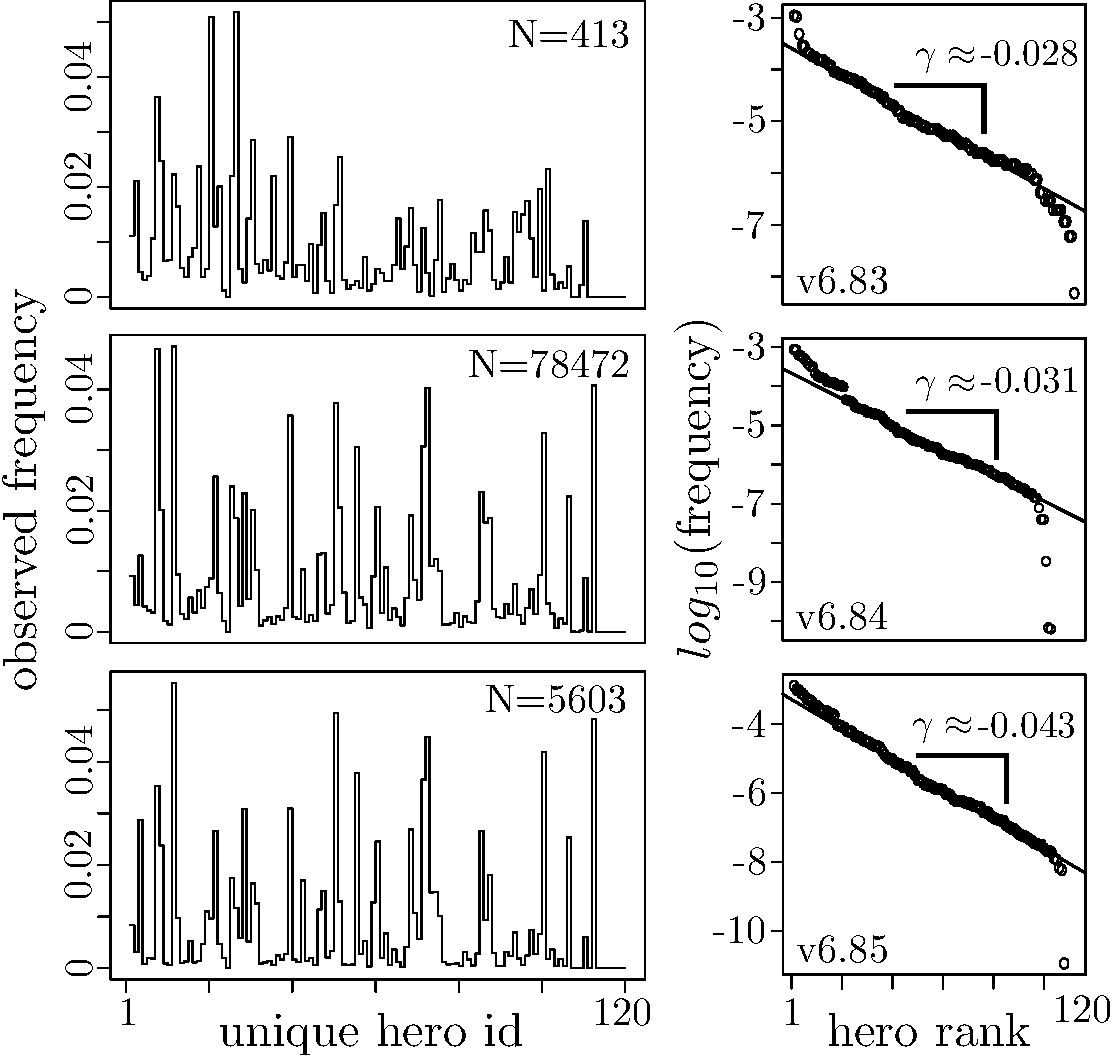
\includegraphics[width=.9\linewidth]{./Figs/hero_usage_across_patches.pdf}}
\caption{Frequency of picks in different patches of DOTA 2. Even if different heroes cease to be used or gain notoriety due to balance changes put forward by the developers of the game (plots on the left), statistical regularities can be observed that survive such changes (right side of the panel). For different patches (from 6.83 at the top to 6.85 at the bottom) we show the hero frequency rank distribution, fitted to an exponential distribution with similar exponents ($\gamma$) across various versions of the game.}\label{frequency_rank_distribution}
\end{figure}

Additionally, we plan to apply the NK landscape framework \cite{Kauffman1987} to the collection of league games. This framework provides a powerful way to formalize the adaptation process given a mapping between a genotype space and the observed phenotype \cite{Levinthal1997}. In our particular dataset these would correspond to team composition (hero picks) and win rates respectively. 

This methodology has proven to be really useful to understand the underlying complexity of many biological processes, such as immunological maturity \cite{Kauffman1989} and cell type differentiation \cite{Kauffman1996} among others. Interestingly, the ruggedness of the fitness landscape is related to the number and intensity of higher order interactions between the different sites in the `genome', tunable in Kauffman's model though the average degree $k$ (Fig.~\ref{landscape}). 

Finding high values of $k$ in the DOTA2 system would imply that heroes have relevant synergies, both positive and negative, that can have a huge impact in the drafting process. Ideally, teams would try to ban positive synergies for the opposing team, while maximizing their own fitness at the same time. However, navigating NK landscapes has been shown to be NP-complete for $k \geq 2$ \cite{Weinberger1996}.

\begin{figure}[h]
\centerline{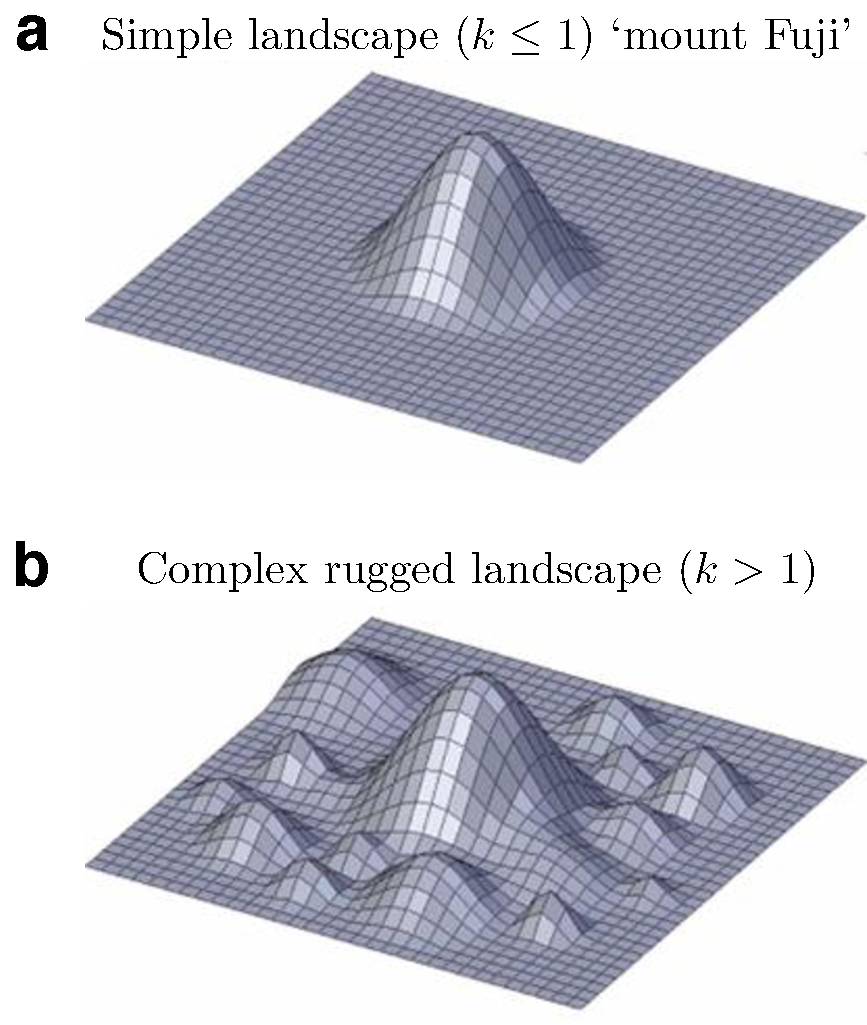
\includegraphics[width=.75\linewidth]{./Figs/landscape.pdf}}
\caption{Fitness landscapes obtained from Kauffman's NK model. At low average connectivity for genome sites \textbf{(a)} the landscape can be navigated, in the sense that a greedy algorithm can easily find the best global strategy. Conversely, as $k$ increases \textbf{(b)}, it becomes increasingly difficult to find the global optimum, instead a greedy algorithm might easily get stuck in a local peak.}\label{landscape}
\end{figure}



\subsection{Characterizing the draft with a hidden Markov model} 


\subsubsection{Model}

Initially, the process was modeled as a Markov Decision Tree. However, due to the massive number of possible states, e.g. 3$^{112}$, corresponding to the 112 characters and the option for unused, picked, or banned for each one, and the 69,464 transitions corresponding to 3,493 games for the pro game data set, the data was insufficient to analyze the data in this manner.

The next step was to coarse grain the heroes into groups based on information from the game. The simplest available method to do this was to use character descriptions from the game itself, which groups the characters into classes of strength, agility, and intelligence. Additionally, each character fills one of nine roles, leading to coarse graining into possibly 27, 9, or 3 groups, which should lead to sufficient state density to perform Hidden Markov Model type analyses.

\subsubsection{Further Analysis}

Once the data is coarse grained into the described groups, a Hidden Markov Model will be generated to describe the underlying strategy of the players in determining their next pick or ban in the draft phase of the game. Additionally, further work into the optimal coarse graining of the characters may yield insights into how they could be grouped for this analysis. Possible unsupervised learning algorithms may be useful for this portion of the analysis.






\subsection{Within Game}

Data from throughout each game was extracted and analyzed in order to determine underlying strategies.  A hidden Markov model was used and is discussed below after an overview of the data processing.  

\subsubsection{Data}

The raw game data was initially downloaded from a DOTA 2 repository in a binary form.  A java parser was written to convert the data into a JSON format, with each event occurring in the game generating an output.  An example for a hero movement event is shown below:
\\
\\
\{``tick":24516,``time":825,``type":``DT\_DOTA\_Unit\_Hero\_X",\\ ``team":3,``x":99,``y":171\}
\\
\\
where `tick' is a subunit of `time', and team indicates 2 or 3 (which must be connected with Dire or Radiant, see below).  The type of event includes position, items, abilities, gold, XP, damage, healing, and death, with each type triggering different tags following the type.  This event-by-event data, which can include multiple events per time step, was transformed into a single time step which keeps track of all events occurring at that step for each hero on each team.  Aggregated statistics for the game a whole, such as which team won and draft order, was folded in with this event data.  The draft order from the aggregated statistics allows the hero names and team number (2 or 3) to be correlated with each team, Dire or Radiant, as the Radiant are denoted as team 0 in the draft.  This is important as the win is denoted as a boolean value for if the Radiant team won or lost, not if team 2 or 3 won or lost.  Figure~\ref{xp} shows an example of the time evolution of one game metric, XP.  This was a fairly unbalanced, fast game in which the Dire team won. 



\begin{figure}[h]
\centerline{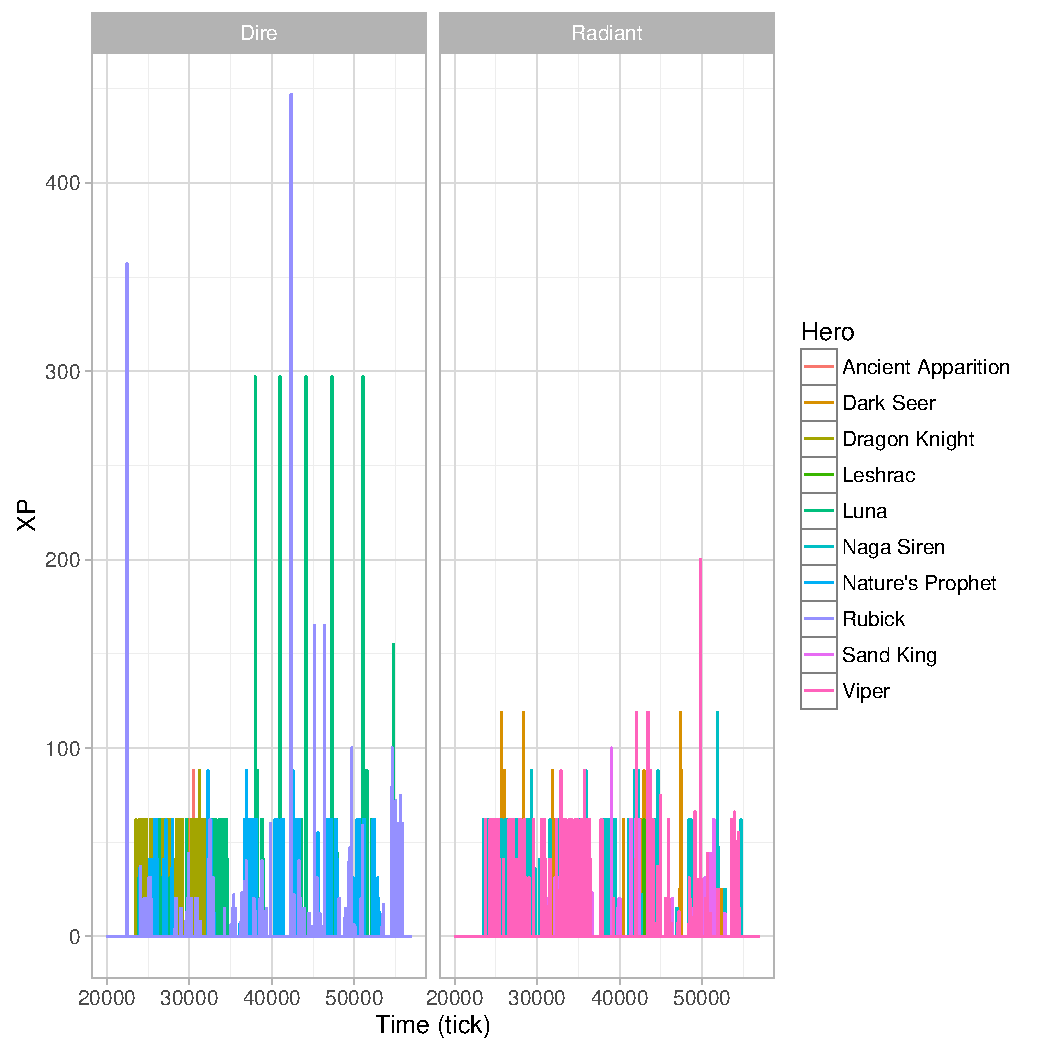
\includegraphics[width=0.8\linewidth]{./Figs/XP_example.pdf}}
\caption{Evolution of experience points, XP, throughout a sample game for each team and hero.}\label{xp}
\end{figure}


\subsubsection{Model}


A hidden Markov model (HMM) was used to explore the latent strategies with DOTA games.  The observed signals were assumed to be observables from the game itself, and the hidden signal was assumed to be the desired strategy. One of the most relevant and revealing observables in the game are the positions of the players.  Fighting is highly correlated with distance, as if two opposing heroes are nearby each other, the probability they will fight is high in order to win the game.  Experience is also accumulated through fighting, and hence, is correlated with distance.  

One method to convert absolute distances of each player into observable states is to coarse grain by relative distance among heroes on a given team.  The states were defined as follows, where the number indicates the number of heroes that are considered ``close" together in a cluster:

\begin{itemize}
\item 1-1-1-1-1
\item 1-1-1-2
\item 1-1-3
\item 1-2-2
\item 2-3
\item 1-4
\item 5
\end{itemize}

For example, the state ``1-1-1-1-1" indicates all heroes are far apart, whereas ``5" denotes heroes are clustered closely together.  ``Closeness" is defined by a relative distance threshold:  if the relative distance between hero A and hero B is below the set threshold, then A and B are considered ``close".  This threshold was set to be 5 units, with the range of the game board being $\sim$ 100 units $\times$ $\sim$ 100 units.  Sensitivity on the hidden states on this threshold was tested and found to be XXXXX.  



\begin{figure}[h]
\centerline{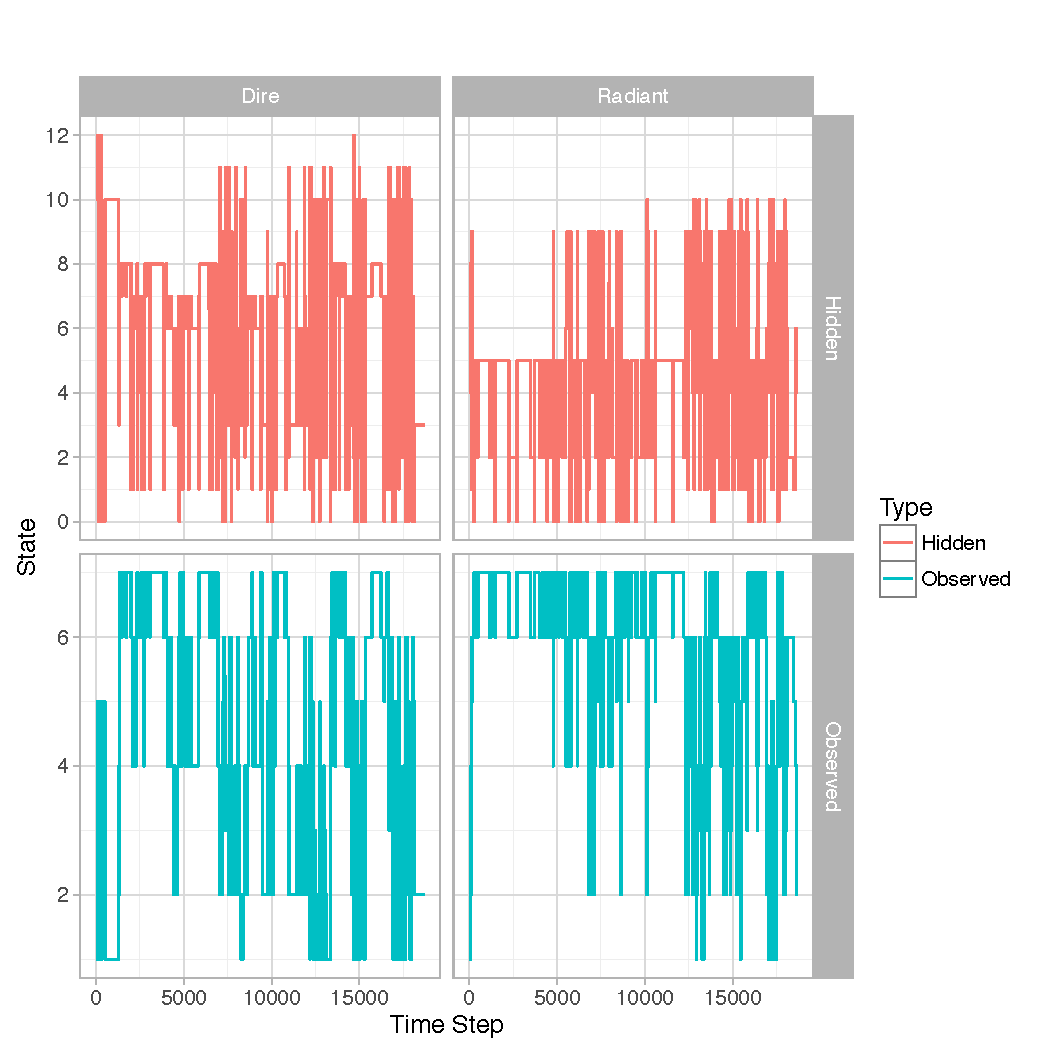
\includegraphics[width=0.8\linewidth]{./Figs/HiddenStatesVsObserved}}
\caption{Evolution of hidden and observed states for a sample game. Note, the hidden state X may not correspond directly to the observed state X.  These numerical labels are arbitrary and used only for plotting purposes.}\label{states}
\end{figure}

The time series of states for a sample game is shown in Fig.~\ref{states}.  For each time step in the game, an observed state was assigned to each team.  This sequence served as an input to the HMM.  The code to estimate the model parameters and the most likely hidden state sequence was provided by Simon DeDeo (http://tuvalu.santafe.edu/$\sim$simon/styled-8/).  The code uses the Akaike information criterion (AIC) in order to estimate the number of hidden states in the model.  For the example game above, the number of hidden states for the Dire team was 13 and 11 for the Radiant, as compared to seven observable states.   

The model that produces the hidden states for the Radiant is shown in Fig.~\ref{model}.

\begin{figure}[h]
\centerline{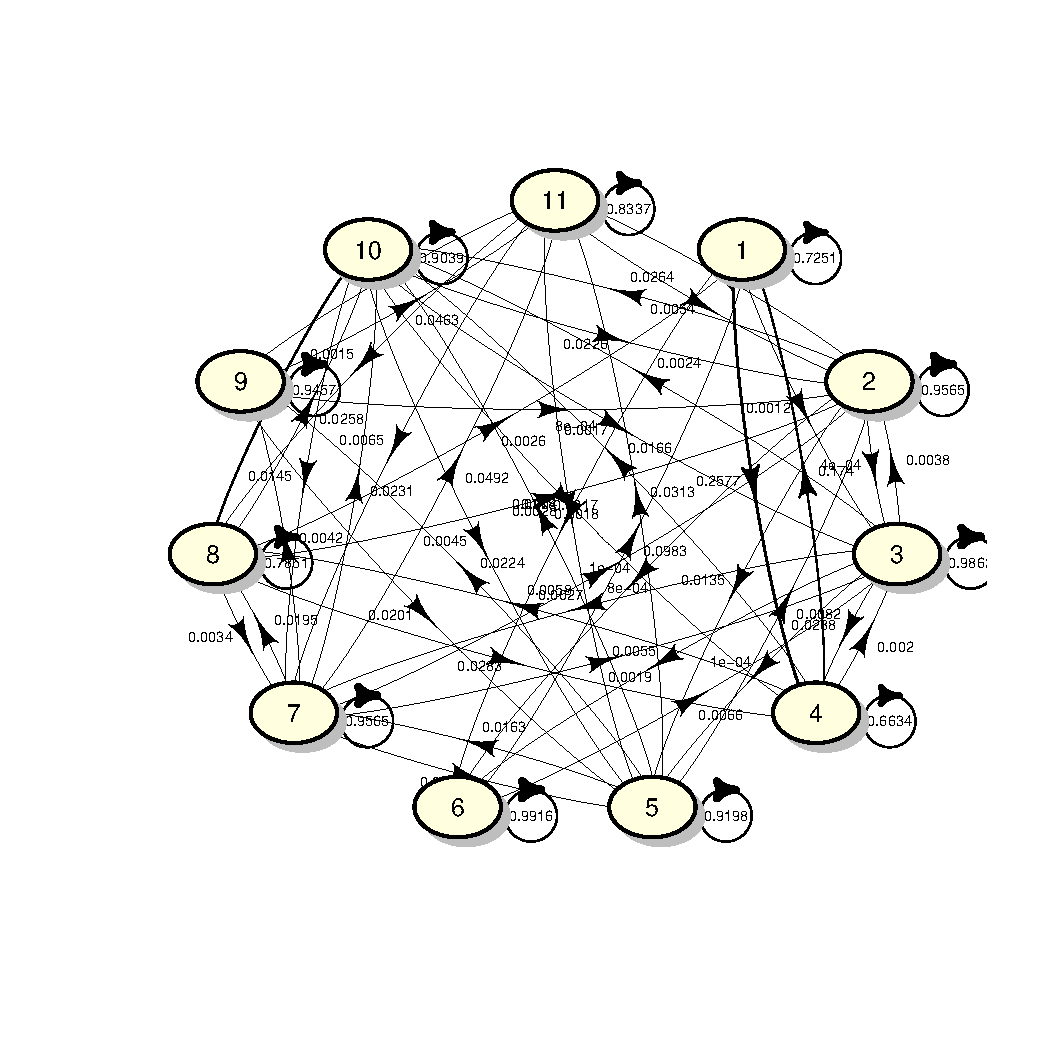
\includegraphics[width=0.8\linewidth]{./Figs/Model.pdf}}
\caption{Hidden Markov model for one team of the sample game.}\label{model}
\end{figure}

Future work will involve unsupervised learning in order to extract the states, using distances within each team (as is done deterministically above), distances among all players, and adding additional features in addition to distances such as XP or gold.  


\subsection{Between Games (Marla)}

Explore why and when players change teams.  Network analysis.  

\section{Conclusions}

X


%----------------------------------------------------------------------------------------
%	APPENDICES (OPTIONAL)
%----------------------------------------------------------------------------------------

%\appendix
%An appendix without a title.

%\appendix[Appendix title]
%An appendix with a title.

%----------------------------------------------------------------------------------------
%	ACKNOWLEDGEMENTS
%----------------------------------------------------------------------------------------

\begin{acknowledgments}
We would like to acknowledge the originator of this idea, David Slater.  Domain knowledge is key.  We would also like to acknowledge Sanith Sanith Wijesinghe, Matt Koehler, and Shaun Michel of the MITRE Corporation; and Simon DeDeo of the Santa Fe Institute for their input and advice.  
\end{acknowledgments}

%----------------------------------------------------------------------------------------
%	BIBLIOGRAPHY
%----------------------------------------------------------------------------------------

%% PNAS does not support submission of supporting .tex files such as BibTeX.
%% Instead all references must be included in the article .tex document. 
%% If you currently use BibTeX, your bibliography is formed because the 
%% command \verb+\bibliography{}+ brings the <filename>.bbl file into your
%% .tex document. To conform to PNAS requirements, copy the reference listings
%% from your .bbl file and add them to the article .tex file, using the
%% bibliography environment described above.  

%%  Contact pnas@nas.edu if you need assistance with your
%%  bibliography.

% Sample bibliography item in PNAS format:
%% \bibitem{in-text reference} comma-separated author names up to 5,
%% for more than 5 authors use first author last name et al. (year published)
%% article title  {\it Journal Name} volume #: start page-end page.
%% ie,
% \bibitem{Neuhaus} Neuhaus J-M, Sitcher L, Meins F, Jr, Boller T (1991) 
% A short C-terminal sequence is necessary and sufficient for the
% targeting of chitinases to the plant vacuole. 
% {\it Proc Natl Acad Sci USA} 88:10362-10366.


%% Enter the largest bibliography number in the facing curly brackets
%% following \begin{thebibliography}
\bibliography{}

\begin{thebibliography}{100}
\bibitem{Kauffman1987}
Kauffman, Stuart, \& Simon Levin. Towards a general theory of adaptive walks on rugged landscapes. {\em Journal of theoretical Biology} 128.1 (1987): 11-45.

\bibitem{Levinthal1997}
Levinthal, Daniel A. Adaptation on rugged landscapes. {\em Management science} 43.7 (1997): 934-950.

\bibitem{Kauffman1989}
Kauffman, Stuart A., and Edward D. Weinberger. The NK model of rugged fitness landscapes and its application to maturation of the immune response. {\em Journal of theoretical biology} 141.2 (1989): 211-245.

\bibitem{Kauffman1996}
Kauffman, Stuart. At home in the universe: The search for the laws of self-organization and complexity. Oxford university press, 1996.

\bibitem{Weinberger1996}
Weinberger, Edward D. Np completeness of kauffman's NK model, a tuneable rugged fitness landscape. No. 96-02-003. 1996.

\end{thebibliography}
\bibliographystyle{unsrt}

%----------------------------------------------------------------------------------------

\end{article}

%----------------------------------------------------------------------------------------
%	FIGURES AND TABLES
%----------------------------------------------------------------------------------------

%% Adding Figure and Table References
%% Be sure to add figures and tables after \end{article}
%% and before \end{document}

%% For figures, put the caption below the illustration.
%%
%% \begin{figure}
%% \caption{Almost Sharp Front}\label{afoto}
%% \end{figure}


%% For Tables, put caption above table
%%
%% Table caption should start with a capital letter, continue with lower case
%% and not have a period at the end
%% Using @{\vrule height ?? depth ?? width0pt} in the tabular preamble will
%% keep that much space between every line in the table.

%% \begin{table}
%% \caption{Repeat length of longer allele by age of onset class}
%% \begin{tabular}{@{\vrule height 10.5pt depth4pt  width0pt}lrcccc}
%% table text
%% \end{tabular}
%% \end{table}

%\begin{table}[h]
%\caption{Table caption}\label{sampletable}
%\begin{tabular}{l l l}
%\hline
%\textbf{Treatments} & \textbf{Response 1} & \textbf{Response 2}\\
%\hline
%Treatment 1 & 0.0003262 & 0.562 \\
%Treatment 2 & 0.0015681 & 0.910 \\
%Treatment 3 & 0.0009271 & 0.296 \\
%\hline
%\end{tabular}
%\end{table}

%% For two column figures and tables, use the following:

%% \begin{figure*}
%% \caption{Almost Sharp Front}\label{afoto}
%% \end{figure*}

%% \begin{table*}
%% \caption{Repeat length of longer allele by age of onset class}
%% \begin{tabular}{ccc}
%% table text
%% \end{tabular}
%% \end{table*}

%----------------------------------------------------------------------------------------

\end{document}